% $Header: /cvsroot/latex-beamer/latex-beamer/solutions/conference-talks/conference-ornate-20min.en.tex,v 1.6 2004/10/07 20:53:08 tantau Exp $

\documentclass[11pt]{beamer}

% This file is a solution template for:

% - Talk at a conference/colloquium.
% - Talk length is about 20min.
% - Style is ornate.

% Copyright 2004 by Till Tantau <tantau@users.sourceforge.net>.
%
% In principle, this file can be redistributed and/or modified under
% the terms of the GNU Public License, version 2.
%
% However, this file is supposed to be a template to be modified
% for your own needs. For this reason, if you use this file as a
% template and not specifically distribute it as part of a another
% package/program, I grant the extra permission to freely copy and
% modify this file as you see fit and even to delete this copyright
% notice. 

\mode<presentation>
{
  % Turn off shadowing, large frame titles, and sans-serif fonts
  % (ALL OF WHICH PISS ME OFF - RBN).
  \usetheme{default}
  \usefonttheme{serif}
  \usecolortheme[RGB={0,0,0}]{structure}
  \setbeamercovered{transparent}
  \setbeamerfont{frametitle}{size=\normalsize,series=\bfseries}
}

\usepackage{graphics}

\usepackage[english]{babel}
% or whatever

%\usepackage[latin1]{inputenc}
% or whatever

\usepackage{times}
\usepackage[T1]{fontenc}
% Or whatever. Note that the encoding and the font should match. If T1
% does not look nice, try deleting the line with the fontenc.

% Add a frame indication to the navigation symbols
\setbeamertemplate{navigation symbols}{}
\setbeamertemplate{footline}{
\vskip1mm \ 
{\it \insertshorttitle}
\hfill
Frame \insertframenumber\ of \inserttotalframenumber\ 
\insertslidenavigationsymbol
\insertframenavigationsymbol
\insertsubsectionnavigationsymbol
\insertsectionnavigationsymbol
\insertdocnavigationsymbol
\insertbackfindforwardnavigationsymbol
\  \vskip1mm
}

\setbeamertemplate{bibliography item}[text]{}

\title[Causality, confounders, and propensity scores] % (optional, use only with long paper titles)
{\textbf{Causality, confounders, and propensity scores}}

\subtitle
{\scriptsize With examples from the Avon Longitudinal Study of Parents and Children (ALSPAC) cohort study at Bristol University, UK
\\ \href{http://www.bristol.ac.uk/alspac/}{\textsl{http://www.bristol.ac.uk/alspac/}}
}

\author[Author, Another] % (optional, use only with lots of authors)
% {F.~Author\inst{1} \and S.~Another\inst{2}}
{
Roger B. Newson
\\ \href{mailto:r.newson@imperial.ac.uk}{r.newson@imperial.ac.uk}
\\ \href{http://www.imperial.ac.uk/nhli/r.newson/}{\textsl{http://www.imperial.ac.uk/nhli/r.newson/}}
}
% - Give the names in the same order as the appear in the paper.
% - Use the \inst{?} command only if the authors have different
%   affiliation.

%\institute[Universities of Somewhere and Elsewhere] % (optional, but mostly needed)
\institute[National Heart and Lung Institute, Imperial College London]
{
National Heart and Lung Institute\\
Imperial College London
}
\date[Asthma Club 2008] % (optional, should be abbreviation of conference name)
{
Presented at Asthma Club, 11~December, 2008
}

\subject{Confounder adjustment}
% This is only inserted into the PDF information catalog. Can be left
% out. 


% If you have a file called "university-logo-filename.xxx", where xxx
% is a graphic format that can be processed by latex or pdflatex,
% resp., then you can add a logo as follows:

% \pgfdeclareimage[height=0.5cm]{university-logo}{university-logo-filename}
% \logo{\pgfuseimage{university-logo}}


%\pgfdeclareimage[height=0.5cm]{university-logo}{university-logo-filename.gif}
%\logo{\pgfuseimage{university-logo}}


\begin{document}

\section{Title page}

\begin{frame}
  \titlepage
\end{frame}

%\begin{frame}
%  \frametitle{Outline}
%  \tableofcontents[pausesections]
%  % You might wish to add the option [pausesections]
%\end{frame}

\section{Definitions}

\begin{frame}
\frametitle{What is causality?}

\begin{itemize}

\item<2-> Suppose $A$ and $B$ are events. ($A$ might be paracetamol exposure, $B$ might be asthma diagnosis.)

\item<3-> Then the statement
$$
\mbox{``A causes B''}
$$
is shorthand for
$$
\mbox{``We can prevent $B$ by \textbf{intervening} to prevent $A$''}.
$$

\item<4-> The event $A$ is known as the \textbf{cause}, and the event $B$ is known as the \textbf{effect}.

\item<5-> Sometimes, $A$ and $B$ are defined as (mean or median) differences, or (mean, median or odds) ratios,
between values of variables.

\item<6-> For instance, $A$ might be a unit increase in Vitamin~D intake (the \textbf{exposure}),
and $B$ might be the corresponding odds ratio for asthma diagnosis (the \textbf{outcome}).

\item<7-> \textit{However}, causality means nothing unless we have a proposed (or fantasized) intervention in mind.

\end{itemize}

\end{frame}

\begin{frame}
\frametitle{What are confounders?}

Confounders are variables other than the outcome and exposure.
There appears not to be a perfect consensus, even among statisticians, on anything else.
\textit{However}, I would propose the following informal criteria:

\begin{itemize}

\item<2-> A confounder is a predictor of ``exposure--proneness''.

\item<3-> A confounder is a predictor of ``outcome--proneness''.

\item<4-> A confounder is expected to be unchanged by the proposed (or fantasized) intervention.

\end{itemize}

\onslide<5->{
All 3 of these criteria may be subject to the prior opinions of the investigators.
\textit{However}, the aim is that subjects with different exposure levels, and identical confounder levels,
should be ``exchangeable'' (Greenland and Robins, 1986\cite{greenland1986}).
}

\onslide<6->{
Note that confounders defined in this way do not have to be ``causally upstream''
from the exposure and outcome, but they should \textit{not} be ``causally downstream'' from either.
(See Hernan \textit{et al.}, 2002.\cite{hernan2002})
}

\end{frame}

\begin{frame}
\frametitle{Candidate confounders are \textit{not} ``innocent until proved guilty''}

\begin{itemize}

\item<2-> In some circles, it is believed that confounders should be excluded from the model,
unless they are \textit{shown} to be ``doing some confounding'',
and predicting the exposure \textit{and} the outcome.

\item<3-> This is typically the principle behind ``stepwise'' procedures,
based \textit{either} on significance levels \textit{or} effect modification,
which were critically reviewed by Greenland (1989)\cite{greenland1989}.

\item<4-> In general, the theory of confidence intervals \textit{does not} cover us
for estimating the parameters in the same data as those in which we found the model.

\item<5-> In particular, a large number of confounders may each have individually unconvincing effects,
which may cumulatively add up to a lot of confounding.

\item<6-> Davey Smith and Ebrahim (2002)\cite{daveysmith2002} argued that inadequate confounder adjustment is probably
more important than ``data--dredging'' in explaining the apparent high rate of ``false positives'' in nutritional epidemiology.

\end{itemize}

\end{frame}

\section{Example from ALSPAC}

\begin{frame}
\frametitle{Example: Dietary scores and asthma in the ALSPAC cohort}

\begin{itemize}

\item<2-> The Avon Longitudinal Study of Parents and Children (ALSPAC) is a birth cohort study,
based at Bristol University, with 14060 subjects, born in the early 1990s.

\item<3-> The \textbf{outcome} of primary interest is doctor--diagnosed asthma at 7 years of age.

\item<4-> The \textbf{exposures} are 5 dietary patterns (or dietary scores),
derived using principal components analysis by Northstone \textit{et al.} (2008)\cite{northstone2008}
from a food frequency questionnaire (FFQ) completed by the mothers during pregnancy.
These scores, expressed in standard deviation (SD) units, were named
``Health--conscious'', ``Traditional'', ``Processed'', ``Confectionery'', and ``Vegetarian''.

\item<5-> The proposed \textbf{interventions} are presumably persuading pregnant mothers to eat a diet
that generally includes more (or less) of health--conscious, traditional, processed, confectionery,
or vegetarian items.

\item<6-> The \textbf{candidate confounder list} was $\ldots$

\end{itemize}

\end{frame}

\begin{frame}
\frametitle{Candidate confounders}

\begin{itemize}

\item<2-> $\ldots$ energy intake, gender, maternal age group, parity, gestational age at birth, prenatal tobacco exposure,
maternal education, maternal housing tenure,
birth weight, head circumference at birth, length at birth,
maternal BMI, maternal ethnic origin, breast feeding in first 6 months, day care in first year,
maternal pre--pregnancy atopic disease history (asthma, eczema, rhinoconjunctivitis),
maternal infection history during pregnancy (colds/flu, urinary, other),
maternal pre--pregnancy migraine history, multiple pregnancy,
paracetamol use in late pregnancy, antibiotic use in late pregnancy, pets in first year, damp in home,
weekend environmental tobacco exposure in first year,
birth season, FFQ completion season, maternal financial difficulties,
younger siblings at 7 years, child's BMI at 7 years.

\item<3-> Most of these are not likely to be ``causally upstream'' from prenatal diet or asthma,
but might indicate aspects of prenatal health or socio--economic state that might influence both.
\textit{However} $\ldots$

\end{itemize}

\end{frame}

\begin{frame}
\frametitle{Candidate confounders (continued)}

\begin{itemize}

\item<2-> $\ldots$ it was thought that an intervention to change maternal diet in pregnancy
might have incidental effects on some of these candidate confounders
(birth weight, head circumference at birth, length at birth,
child's BMI at 7 years).

\item<3-> \textit{Therefore}, we also defined a ``non--causal'' confounder set,
excluding these particular confounders.

\item<4-> So we had 3 nested alternative confounder sets:  ``None'' (unadjusted),  ``Non--causal'', and ``All''.

\end{itemize}

\end{frame}

\section{Propensity scores}

\begin{frame}
\frametitle{Problem: The confounder space potentially has an infinite number of dimensions!}

\begin{itemize}

\item<2-> The number of possible combinations of confounder values increases \textit{exponentially} with the number of confounders,
with each combination representing a small number of subjects.

\item<3-> It is therefore not practicable to compare only subjects with exactly the same confounder values.

\item<4-> Assuming a linear, additive model causes parameter numbers to increase \textit{linearly} with the number of confounders.

\item<5-> \textit{However}, the number of parameters may still be uncomfortably large,
possibly affecting the validity of the Central Limit Theorem.

\item<6-> We would like to reduce the potentially infinite--dimensional confounder space to a manageable number of groups,
within which subjects with different exposure levels are comparable.

\end{itemize}

\end{frame}

\begin{frame}
\frametitle{Part of a solution: Propensity scores}

\begin{itemize}

\item<2-> A \textbf{propensity score} (Imai and Van Dyk, 2004\cite{imai2004})
is a measure of the ``exposure--proneness'' of a subject,
based on the confounder values.

\item<3-> It is defined by fitting a statistical model, predicting the exposure from the confounders.

\item<4-> For each subject, the propensity score is equal to the predicted exposure level for that subject,
or sometimes to the corresponding linear predictor.

\item<5-> Usually, we then group the subjects into a manageable number of similar--sized groups,
based on their propensity scores.

\item<6-> Having found our grouping in the exposure and confounder data, we can then estimate within--group effects of exposure on outcome,
based on the within--group association of the outcome variable with the exposure variable.

\end{itemize}

\end{frame}

\begin{frame}
\frametitle{Example: Dietary scores and asthma in the ALSPAC cohort}

\begin{itemize}

\item<2-> In the ALSPAC cohort, the mothers of 12008 children completed the food frequency questionnaire (FFQ),
and the 5 dietary pattern scores (``Health--conscious'', ``Traditional'', ``Processed'', ``Confectionery'', and ``Vegetarian'')
were computed.

\item<3-> For each combination of the 5 diet scores and the 2 non--empty confounder sets (``All'' and ``Non--causal''),
a linear regression model was fitted, predicting the diet score from the confounder set.

\item<4-> The propensity score for each diet score, based on each confounder set,
was the predicted value of that diet score, based on the regression model with those confounders.

\item<5-> The 12008 children were grouped into 64 nearly--equal propensity groups,
based on the appropriate propensity score.

\item<6-> We then fitted a logistic regression model for the outcome ``Doctor--diagnosed asthma''
(recorded for 7625 subjects),
with 64 baseline odds (1 per propensity group), and a common odds ratio for asthma per SD of the diet score.

\end{itemize}

\end{frame}

\begin{frame}
\frametitle{Odds ratios for asthma per standard--deviation change in diet scores}

\begin{columns}[t]
\begin{column}{48mm}
\begin{itemize}
\item<2-> Increasing the ``Healthy'' score by 1 SD seems to predict a modest fall in asthma odds (OR=0.90).
\item<3-> But if we compare only ``comparable'' subjects, the OR is closer to 1,
and the confidence interval is wider.
\item<4-> \textit{Therefore}, the association \textit{may} arise because more
``Healthy--diet--prone'' subjects are also less ``asthma--prone'',
whatever their mothers eat.
\end{itemize}
\end{column}
\begin{column}[T]{80mm}
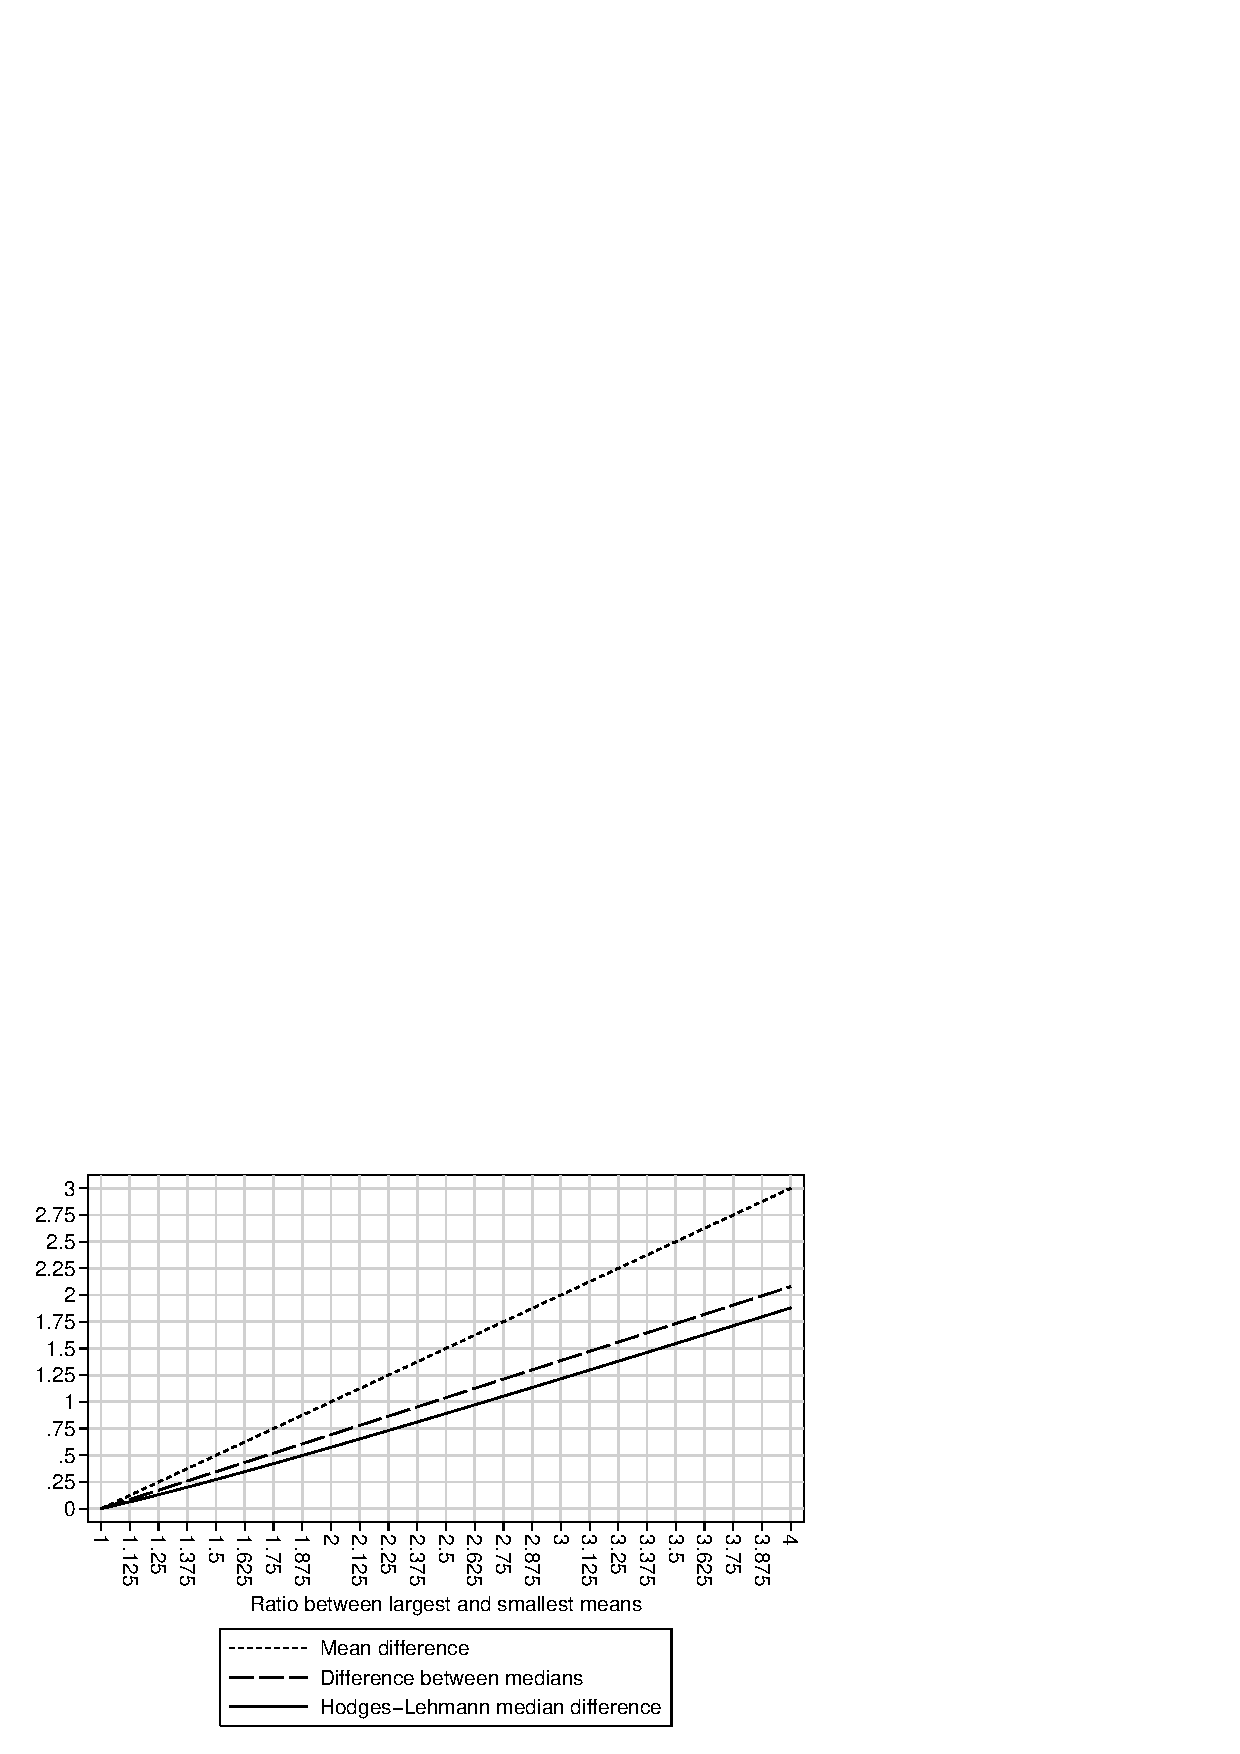
\includegraphics[width=76mm]{figseq1.pdf}
\end{column}
\end{columns}

\end{frame}

\section{Advantages of propensity scores}

\begin{frame}
\frametitle{Advantages of propensity scores}

\begin{itemize}

\item<2-> Statistical methods assume 2 ``quasi--independent'' stages in an analysis:
``Choosing the parameters to estimate'' and ``Estimating the parameters''.

\item<3-> It is \textit{implicitly assumed} that we find the model in a different set of data
from the dataset used to estimate its parameters.

\item<4-> Using propensity groups, we find the model in the exposure and confounder data,
and measure its parameters in the outcome data.

\item<5-> The confidence interval formulas are based on the conditional distribution of the outcomes,
given the exposures and confounders.

\item<6-> This rigorous separation of the 2 stages implies that we can do various ``interactive'' checks
on the joint distribution of the exposure, confounders and propensity groups,
\textit{before} looking at the outcomes. For example $\ldots$

\end{itemize}

\end{frame}

\begin{frame}
\frametitle{Choosing the number of propensity groups}

\begin{itemize}

\item<2-> Given an exposure, and a candidate confounder list,
we would like to choose a sensible number of propensity groups.

\item<3-> If there are too few, then there will be residual confounding.

\item<4-> If there are too many, then there will be too few within--group comparisons
between subjects with different exposure levels (losing power).

\item<5-> The power of the propensity score to predict the exposure may be measured by calculating
Somers'~$D$ of the propensity score with respect to the exposure (Newson, 2006\cite{newson2006}).

\item<6-> Somers'~$D$ has a standard unstratified version,
including all pairs of subjects with different exposure levels.

\item<7-> It also has a stratified version,
restricted to pairs of subjects with different exposure levels within the same propensity group.

\end{itemize}

\end{frame}

\begin{frame}
\frametitle{Example: Diet scores in the ALSPAC study}

\begin{itemize}

\item<2-> We wanted to choose a sensible number of propensity groups
to stratify the propensity score for each diet score.

\item<3-> For each of the 5 diet scores,
we used the unstratified Somers'~$D$ of its propensity score with respect to the diet score
to measure the power of the confounders (collectively) to predict the diet score.

\item<4-> We used the group--stratified Somers'~$D$ to measure the same predictive power,
\textit{within} propensity groups.

\item<5-> We tried various numbers of propensity groups, from 2 to 128.

\item<6-> Increasing the number of propensity groups decreased the stratified Somers'~$D$.
With 64 propensity groups, little of the original association remained.

\end{itemize}

\end{frame}

\begin{frame}
\frametitle{Predictive power of the propensity scores for the ``Non--causal'' confounder list}

\begin{columns}[t]
\begin{column}{48mm}
\begin{itemize}
\item<2-> The unstratified Somers'~$D$ values show that the counfounders predict the diet scores.
(But not \textit{too} well.)
\item<3-> The stratified Somers'~$D$ values show that, within 64 propensity groups,
this predictive power is not much of a problem.
\item<4-> \textit{Therefore}, 64 propensity groups should be sufficient for modelling out confounding.
\end{itemize}
\end{column}
\begin{column}[T]{80mm}
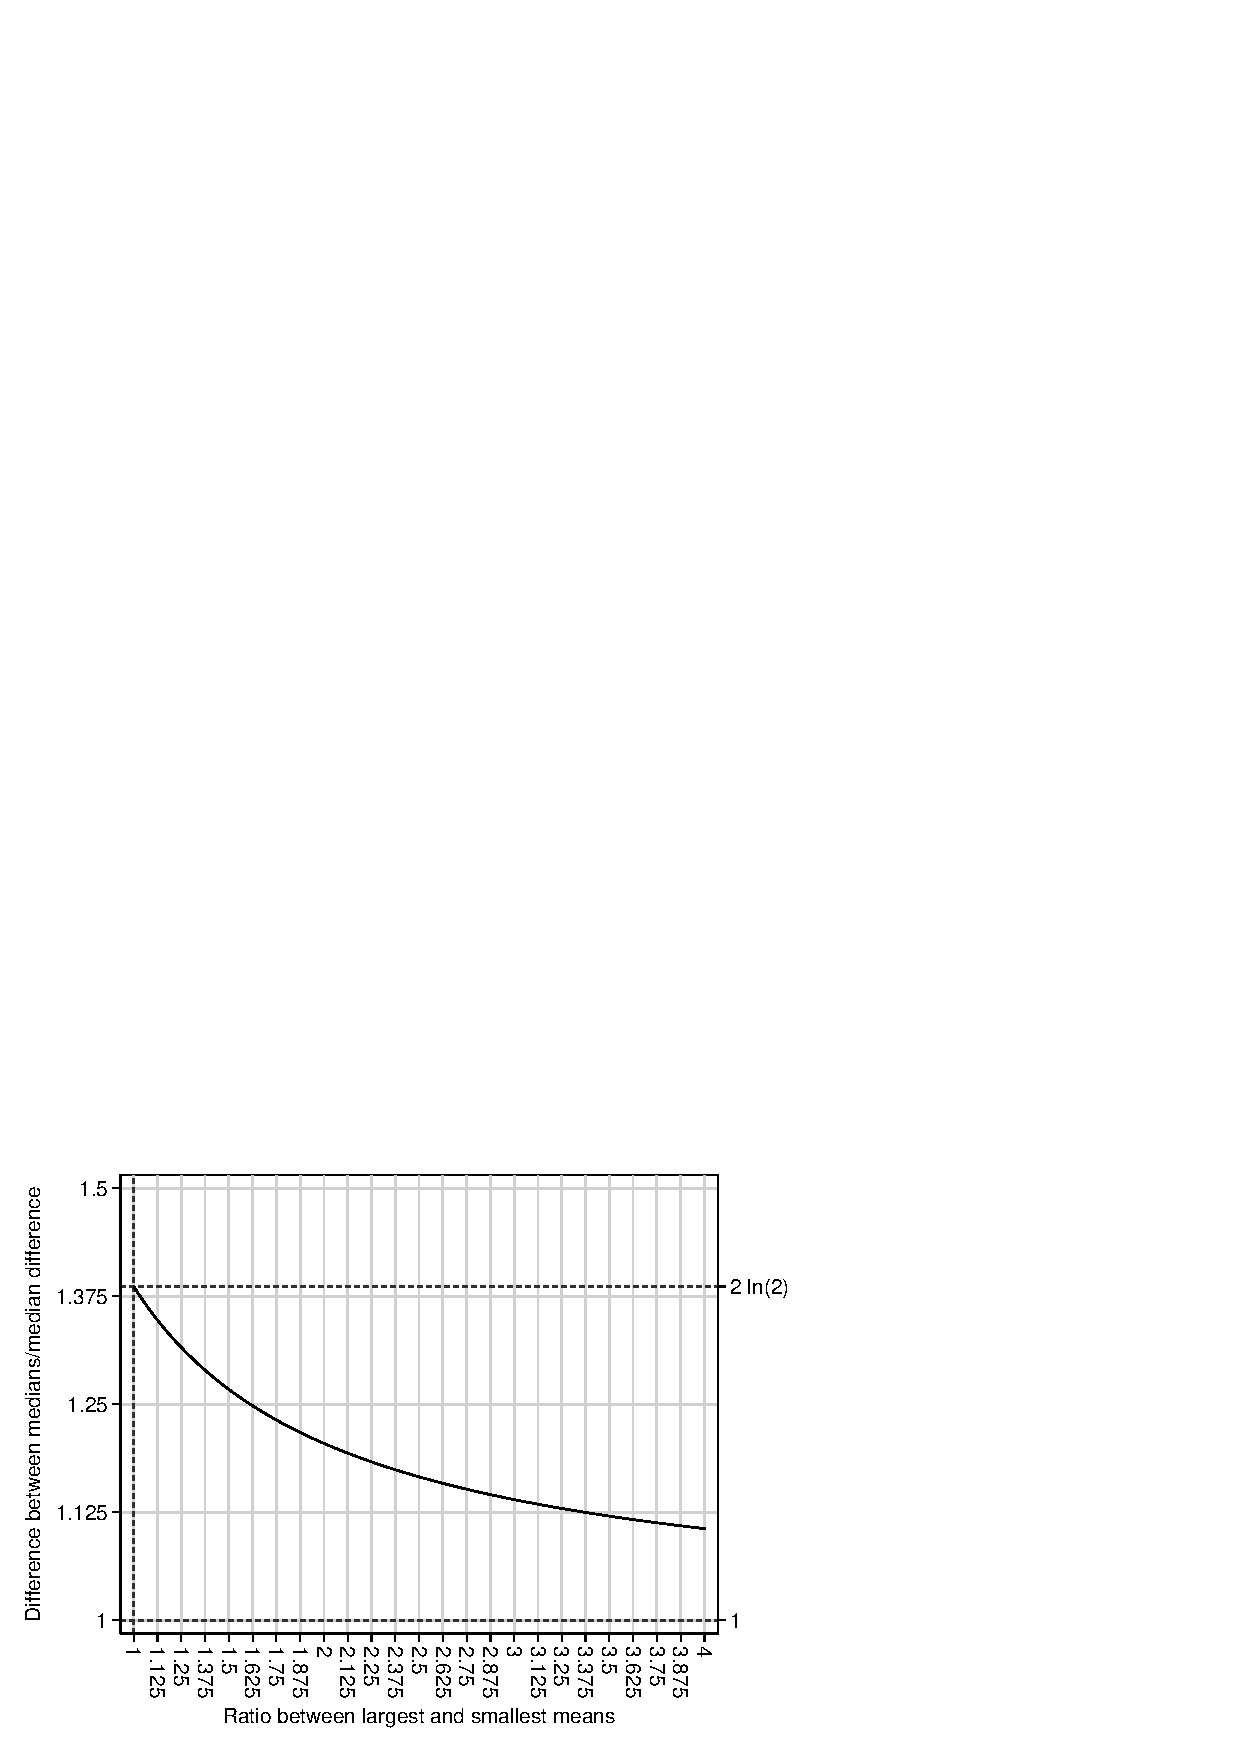
\includegraphics[width=76mm]{figseq2.pdf}
\end{column}
\end{columns}

\end{frame}

\section{Limitations of propensity scores}

\begin{frame}
\frametitle{Limitations of propensity scores}

\begin{itemize}

\item<2-> Propensity scores cannot control for \textit{unobserved} confounders. (Nor can most alternatives.)

\item<3-> Propensity scores do not tell us which confounders are ``doing the confounding''. (Nor can most alternatives, most of the time.)

\item<4-> \textit{However}, their \textit{fundamental} limitation is that they only measure the ``exposure--proneness'' aspect of confounding.

\item<5-> If we have prior reason to believe that a concomitant variable predicts ``outcome--proneness'' \textit{within} each propensity group,
then there is a case for including that concomitant variable, in addition to the propensity score.

\item<6-> This can gain power by reducing residual variation.
The concomitant variable is then acting as a blocking factor,
rather than as a confounder properly so called.

\end{itemize}

\end{frame}

\begin{frame}
\frametitle{Example: Height, gender, and lung function outcomes}

\begin{itemize}

\item<2-> In asthma research, outcomes are often lung function measures.

\item<3-> Whatever exposure we are interested in,
we are confident, \textit{a priori}, that height and gender will predict lung function well,
even within each exposure--propensity group.

\item<4-> We therefore usually adjust for height and gender,
whether or not these were included in calculating the propensity score.

\item<5-> In fact, we are so confident that height and gender have an effect,
that we usually use a \textit{preliminary} regression model of lung function with respect to height and gender,
and then enter the lung function outcome into the \textit{main} analysis as a standardized residual.

\item<6-> Note that we are not worried by the possibility
that taller children have higher vital capacity only because their mothers were better fed.

\end{itemize}

\end{frame}

\section{Over--adjusting}

\begin{frame}
\frametitle{What do we mean by ``over--adjusting''?}

\onslide<2->{
It is not always clear what is meant by this, except that we should have adjusted for fewer confounders.
\textit{However}, I would argue that it can mean one of two things:
}

\begin{itemize}

\item<3-> \textbf{Some of the confounders are causally downstream from the proposed intervention.}
For instance, if we think the proposed dietary intervention during pregnancy will have the side effects
of making children less small at birth, or less fat at 7 years,
then we should not estimate its effect by comparing children with different maternal diets
and the same birth weight and BMI.

\item<4-> \textbf{The confounders collectively predict the exposure ``too well''.}
This may happen if the number of confounders becomes too close to the number of subjects,
and can cause loss of power.
This should be checked by measuring the association between the exposure and the propensity score,
using scatter plots and/or Somers'~$D$ and/or other methods being developed.
If this is a problem, then we need to use a less ambitious confounder set.

\end{itemize}

\end{frame}

\section{Summary}

\begin{frame}
\frametitle{Summary}

\begin{itemize}

\item<2-> Causal arguments are meaningless, unless we have an intervention in mind.

\item<3-> Confounders must be variables that we do not expect to be changed by that intervention,
and may (collectively) indicate ``exposure--proneness'' and ``outcome--proneness''.

\item<4-> Usually, we cannot compare only subjects with \textit{identical} confounder values,
so we have to reduce the number of confounder groups somehow.

\item<5-> Propensity scores are a good method for grouping the confounder value combinations by exposure--proneness.

\item<6-> \textit{However}, we can gain more power if we \texit{also} know of ways to adjust for outcome--proneness,
within each propensity group.

\end{itemize}

\end{frame}

\section{References}

\begin{frame}
\frametitle{References}

\setbeamerfont{text}{size=\small}

{\scriptsize

\begin{thebibliography}{10}

\bibitem{daveysmith2002}
Davey Smith G, Ebrahim S.
Data dredging, bias or confounding. They can all get you into the BMJ and the Friday papers.
\textsl{British Medical Journal} 2002; \textbf{325}: 1437--1438.

\bibitem{greenland1986}
Greenland S, Robins JM.
Identifiability, exchangeability , and epidemiological confounding.
\textsl{International Journal of Epidemiology} 1986; \textbf{15(3)}: 413--419.

\bibitem{greenland1989}
Greenland S.
Modelling and variable selection in epidemiologic analysis.
\textsl{American Journal of Public Health} 1989; \textbf{79(3)}: 340--349.

\bibitem{hernan2002}
Hernan MA, Hernandez--Diaz S, Werler MM, Mitchell AA.
Causal knowledge as a prerequisite for confounding evaluation:
an application to birth defects epidemiology.
\textsl{American Journal of Epidemiology} 2002; \textbf{155(2)}: 176--184.

\bibitem{imai2004}
Imai K, van Dyk DA.
Causal inference with general treatment regimes: generalizing the propensity score.
\textsl{Journal of the American Statistical Association} 2004; \textbf{99(467)}: 854--866.

\bibitem{newson2006}
Newson R.
Confidence intervals for rank statistics: Somers'~$D$ and extensions.
\textsl{The Stata Journal} 2006; \textbf{6(3)}: 309--334.

\bibitem{northstone2008}
Northstone K, Emmett P, Rogers I.
Dietary patterns in pregnancy and associations with socio-demographic and lifestyle factors.
\textsl{European Journal of Clinical Nutrition} 2008; \textbf{62}: 471--479.

\end{thebibliography}

}

\bigskip

\end{frame}

\end{document}
